%%%%%%%%%%%%%%%%%%%%%%%%%%%%%%%%%%%%%%%%%%%%%%%%%%%%%%%%%%%%%%%%%%%%%%%%%%%%%%
%
% PRÉAMBULE
%
%

% LaTeX 2e sinon rien !
\NeedsTeXFormat{LaTeX2e}

% C'est un rapport...
\documentclass[a4paper,11pt]{report}

% Style du document : personnalisé si disponible, sinon LaTeX par défaut
\newif\ifbglstyle
\IfFileExists{bglstyle.sty}{
  \usepackage{bglstyle} % Mon identité visuelle ;-)
  \bglstyletrue
}{
  \bglstylefalse
}

\ifbglstyle\else
  % Packages de base
  \usepackage[utf8]{inputenc}
  \usepackage[T1]{fontenc}
  \usepackage{ifpdf,textcomp,ae,aecompl,aeguill}
  \usepackage[margin=3cm]{geometry}

  % Commandes définies ici pour assurer la compatibilité avec le style perso
  \makeatletter
  \renewcommand{\title}[1]{\renewcommand{\@mytitle}{#1}}
  \newcommand{\@mytitle}{}
  \newcommand{\subtitle}[1]{\renewcommand{\@title}{\@mytitle\\#1}}
  \newcommand{\group}[1]{}
  \newcommand{\entity}[1]{}
  \makeatother

  % Si jamais le rendu du style LaTeX standard diffère légèrement du style
  % personnalisé, ça ne produira pas d'avertissement (overful/underful hbox)
  \sloppy
\fi

% Packages supplémentaires utilisés par ce document
\usepackage{graphicx}
\usepackage[french,english]{babel}

% Informations sur le document
\title{Rapport de projet Mobilité et Réseaux Sans Fil : CWP}
\author{Benjamin Gaillard, Lionel Imbs, Guillaume Lacroix}
\date{21 février 2007}
\group{Master 2 RIA}
\entity{\includegraphics[keepaspectratio,height=1.5cm]{images/ulp}}

% Hyperlinks
\ifpdf
  \usepackage[pdftex,bookmarks,bookmarksopen,bookmarksnumbered,%
              pdfstartview=Fit,pdfview=FitH]{hyperref}
  \makeatletter
  \hypersetup{%
    pdftitle  = {\@title},
    pdfauthor = {\@author},
    pdfborder = {0 0 0}
  }
  \makeatother
  \usepackage{thumbpdf}
\else
  \usepackage[dvips]{hyperref}
\fi

% Redéfinition d'une information (pour la présentation)
\title{%
  \vspace*{3cm}%
  {\large Mobilité et Réseaux Sans Fil}\\
  CWP : portail web captif%
}
\subtitle{%
  Rapport%
  \vspace{2cm}%
  \begin{center}%
    
\includegraphics[keepaspectratio,width=0.7\textwidth]{images/cwp}%
  \end{center}%
}
\author{%
  Benjamin \textsc{Gaillard}\\%
  Lionel \textsc{Imbs}\\%
  Guillaume \textsc{Lacroix}%
}

% Commandes personnalisées
\newcommand{\ensp}[1]{\selectlanguage{english}#1\selectlanguage{french}}
\newcommand{\strong}[1]{\textbf{#1}}
\newcommand{\file}[1]{\ensp{\textsf{#1}}}
\newcommand{\var}[1]{\ensp{\textit{#1}}}
\newcommand{\type}[1]{\ensp{\texttt{#1}}}
\newcommand{\func}[1]{\ensp{\textsf{#1}}}
\newcommand{\class}[1]{\ensp{\textsf{#1}}}
\newcommand{\code}[1]{\ensp{\texttt{#1}}}
\newcommand{\bs}{\textbackslash}

% Commandes pour ce rapport
\newcommand{\cwp}{%
  %\includegraphics[keepaspectratio,height=0.55\normalbaselineskip]%
  %                {images/cwp-text}%
  CWP%
}
\newcommand{\portalurl}{portal.cwp}
\newcommand{\portal}{\href{http://\portalurl/}{\ensp{\file{\portalurl}}}}


%%%%%%%%%%%%%%%%%%%%%%%%%%%%%%%%%%%%%%%%%%%%%%%%%%%%%%%%%%%%%%%%%%%%%%%%%%%%%%
%
% CONTENU (enfin !)
%
%

\begin{document}

\selectlanguage{french}
\maketitle
\tableofcontents
%\listoffigures

\setlength{\parskip}{0.3\normalbaselineskip}

\chapter{Introduction}

Pour autoriser des clients à se connecter à un réseau sans fil, il existe
plusieurs alternatives. L'une d'entre-elles est le portail web captif qui
a l'avantage de donner accès à une partie du réseau (pouvant se limiter au
portail lui-même uniquement) avant que l'authentification n'ait lieu. Cela
autorise la mise en place d'un accès pour des personnes n'ayant pas besoin de
connaître leurs informations d'authentification avant de pouvoir se connecter.
Elles peuvent ainsi créer leur compte sur place, valider une charte
d'utilisation, obtenir des informations pour configurer leur poste client,
etc\dots

Au jour d'aujourd'hui il est nécessaire de prendre en compte le protocole IPv6
qui remplacera l'actuel IPv4 dans un avenir proche. Les solutions de portail
web captif existantes ne proposent pas un tel support. Il est donc nécessaire
de modifier l'existant ou de créer un nouveau portail. Nous avons choisi cette
dernière solution car elle permet une prise en charge totalement intégrée
d'IPv6. De plus, vous avons pu créer un portail gérant plus de services que la
plupart des solutions existantes actuellement.

Nous allons donc présenter dans ce rapport le portail web captif que nous
avons écrit. Nous l'avons appelé \cwp, pour \emph{Captive Web Portal}.


\chapter{Fonctionnalités}

Dans cette partie, nous allons présenter les fonctionnalités que nous avons
implémentées dans \cwp{} ainsi que les choix techniques que nous avons eus à
effectuer.

\section{Implémentation}

\cwp{} a été écrit en PHP 5. Notre choix s'est porté sur ce langage de script
pour plusieurs raisons :
\begin{itemize}
  \item possibilité d'écrire du code orienté objet ;
  \item omniprésence du langage : du fait de l'utilisation très répandue de
        PHP (une grande partie des sites web dynamiques), ce langage est
        facile d'accès et son installation doit être aisée quel que soit le
        système utilisé ;
  \item intégration à Apache : contrairement aux scripts \textsc{cgi} (Perl,
        Bash\dots), PHP peut être utilisé sous forme d'extension à Apache ce
        qui lui permet d'être résident en mémoire ; il n'est pas entièrement
        rechargé à chaque exécution d'un script. L'avantage direct est la
        possibilité d'utiliser \cwp{} sur des systèmes limités en ressources
        tels que des routeurs.
\end{itemize}\medskip

De plus, \cwp{} adopte une architecture modulaire : il peut ainsi être
facilement étendu et/ou porté sur d'autres systèmes, en définissant juste
de nouvelles classes basées sur les interfaces existantes. Il est notamment
possible de rajouter des services, des méthodes d'authentification, le support
d'un autre firewall, etc., de manière simple et rapide. Il est même prévu de
pouvoir rajouter de nouveaux protocoles (ceux actuellement gérés étant
Ethernet, IPv6 et IPv4). \cwp{} est donc prêt pour de futures évolutions.

\section{Sécurité}

L'implémentation de \cwp{} a été réalisée avec la sécurité comme facteur
primordial. Le portail étant exécuté à travers Apache et devant avoir accès
aux tables du \emph{firewall}, il était nécessaire de trouver une solution qui
permette la manipulation de ces tables sans avoir besoin de faire tourner le
portail sous l'identité du superutilisateur \emph{root}.

Pour ce faire, un \emph{wrapper} a été écrit. Ce dernier permet d'exécuter les
commandes \func{iptables}, \emph{ip6tables} et \emph{ebtables} sous l'identité
d'Apache mais n'autorisent la manipulation que de certaines tables : celles
dont le nom commence par \og cwp\_\fg. Le portail peut ainsi modifier ses
propres règles tout en n'ayant pas accès aux autres tables du pare-feu.

\section{Services utilisés}

\cwp{} nécessite les éléments suivants pour fonctionner :
\begin{itemize}
  \item un système d'exploitation basé sur le noyau Linux : le fonctionnement
        du portail repose sur Netfilter --- commandes \func{iptables} et
        \func{ip6tables} --- pour les autorisation d'accès et la redirection
        sur la page web du portail ; cependant \cwp{} peut être aisément porté
        sur un autre système du fait de son implémentation modulaire ;
  \item \func{ebtables}, si l'on a l'intention d'utiliser un pont réseau (voir
        la section suivante pour plus de détails) ;
  \item \file{iproute2} pour Linux (successeur d'\func{ipconfig}), pour la
        récupération et l'application de paramètres liés aux interfaces
        réseau ;
  \item Apache, avec les modules \file{mod\_rewrite} et si possible
        \file{mod\_ssl} ;
  \item PHP 5 : les fonctionnalités objet de la version 5 sont requises, les
        version antérieures ne sont pas supportées. Le module POSIX est
        obligatoire ainsi que le module PECL RADIUS si cette méthode
        d'authentification est utilisée ;
  \item optionnellement, les serveurs Bind (DNS), RADVD (annonce de routeur
        IPv6) et DHCPD (DHCP pour IPv4), suivant les besoins.
\end{itemize}\medskip

\cwp{} est capable de configurer et de lancer automatiquement des serveurs
additionnels. Ceux-ci incluent un serveur DNS (servant de cache et permettant
de résoudre l'adresse spéciale \portal), un annonceur de routeur IPv6 pour
l'autoconfiguration des adresses IPv6 et un serveur DHCP pour l'attribution
des adresses IPv4. Si les exécutables de ces serveurs sont présents sur le
système, \cwp{} les utilise par défaut.

\section{Support réseau}

Il est possible de faire fonctionner \cwp{} sur un pont (\emph{bridge}),
permettant ainsi de laisser la tâche de l'attribution des adresses à un autre
routeur déjà présent sur le réseau. À noter que cela peut être fait de manière
indépendante pour IPv4 et IPv6 ; par exemple, il est tout à fait possible que
l'adresse IPv4 soit attribuée par notre propre serveur DHCP mais que l'adresse
IPv6 soit annoncée par un autre routeur, y compris si un autre serveur DHCP
est déjà présent.

Le portail peut être accédé en utilisant son adresse IP ou l'adresse spéciale
\portal{} (si un serveur DNS est disponible et activé). Si l'authentification
n'a pas encore eu lieu, le client sera de toute manière automatiquement
redirigé vers le portail s'il tente d'accéder à un autre site.

Dans le cas où c'est \cwp{} qui attribue les adresses, il va se baser sur les
adresses déjà définies sur l'interface connectée au sous-réseau qu'il devra
gérer. Si une adresse n'est pas encore définie, une adresse automatique sera
automatiquement ajoutée (adresse privée pour IPv4, adresse \emph{site-local}
pour IPv6, générées aléatoirement pour éviter une éventuelle collision avec
une adresse déjà existante). Si ce n'est pas ce que l'on souhaite, il suffit
de définir manuellement les adresses souhaitées avant le démarrage de \cwp.

Dans le cas où un pont est utilisé, celui-ci devra utiliser deux adresses pour
chaque protocole : la première définie sera considérée comme étant celle du
réseau interne, la seconde étant utilisée pour le sous-réseau dont le portail
a la charge.

\section{Filtrage et redirection}

Par défaut, \cwp{} n'autorise l'accès qu'aux services suivant avant
authentification, le reste du trafic étant purement et simplement supprimé :
\begin{itemize}
  \item sollicitation de voisin et de routeur IPv6 ;
  \item requêtes DHCP ;
  \item serveur(s) DNS ;
  \item le serveur web (HTTP et HTTPS) du portail.
\end{itemize}\medskip

L'accès au service web (HTTP) de n'importe quelle adresse autre que celle du
portail génèrera une redirection vers le portail. Ainsi chaque tentative
d'accès à un site Internet sera interceptée si l'authentification n'a pas
encore été réalisée avec succès.

Il est possible de configurer \cwp{} pour autoriser d'autres services sur
d'autres machines avant que l'authentification n'ait eu lieu. Une fois
celle-ci passée avec succès, l'accès au reste du réseau est autorisé. Pour
configurer de manière fine le filtrage après authentification, il convient
d'utiliser les commandes \func{iptables} et \func{ip6tables}, cela n'étant pas
géré par \cwp{} : en effet, cela serait redondant d'autant que l'utilisation
des commandes sus-mentionnées permettent la réalisations de configurations
bien plus puissantes et personnalisées, gérer toutes les fonctionnalités de
Netfilter n'était pas le rôle de \cwp.

\section{Installation}

\cwp{} étant basé sur les GNU Autotools, l'installation relève d'un
classique :\\\verb!./configure && make && make install!.

Une fois le paquet installé, il convient de configurer Apache pour qu'il
puisse fonctionner avec. Un fichier d'exemple de configuration est livré avec.
De même, si l'on veut pouvoir lancer les services associés au démarrage, il
est recommandé d'écrire les scripts correspondant. Cela étant spécifique à
chaque distribution, le script n'a pas été créé.

Cependant, les fichiers nécessaires à un bon fonctionnement sous une
distribution Gentoo Linux sont fournis, incluant l'\emph{ebuild}. En utilisant
ce fichier, on peut donc installer \cwp{} en tapant la commande
\og\verb!emerge net-misc/cwp!\fg.

Il est préférable d'ajuster les paramètres (\emph{USE flags}) suivant ce que
l'on désire installer/utiliser. L'\emph{ebuild} se charge lui-même de
configurer Apache et de créer une clé autosignée pour le fonctionnement
d'Apache avec SSL (serveur web HTTPS).

\textbf{Note} : il est recommandé d'utiliser un accélérateur PHP tel
qu'eAccelerator pour une exécution plus rapide des scripts du portail.


\chapter{Fichiers}

Dans cette partie, nous allons décrire les différents fichiers composant le
projet : l'organisation de l'archive, les fichiers source PHP et les fichiers
de configuration.

\section{Organisation de l'archive}

Les sources de \cwp{} sont réparties dans différents répertoire suivant leurs
fonctions. Il s'agit des répertoires suivant :
\begin{itemize}
  \item \file{doc-fr} : la documentation française (ce rapport) ;
  \item \file{etc} : fichiers de configuration et scripts de démarrage
        génériques ;
  \item \file{gentoo} : l'\emph{ebuild}, la configuration d'Apache et le
        script de démarrage pour une distribution Gentoo ;
  \item \file{htdocs} : les fichiers utilisés pour l'interface web (feuille de
        style, images) ;
  \item \file{php} : les sources du portail, en PHP 5 orienté objet ;
  \item \file{wrapper} : les \emph{wrappers} pour \file{iptables},
        \file{ip6tables} et \file{ebtables} (voir la section sur la sécurité
        pour connaître leur utilité).
\end{itemize}

\section{Fichiers source PHP}

Les sources PHP sont organisées de telle façon qu'à une classe \og de
base\fg{} corresponde un fichier. Par classe \og de base\fg, nous entendons
les classes qui n'héritent pas d'une autre. Ainsi, par exemple, la classe
\type{Portal} réside seule dans un fichier et les classes \type{Address},
\type{Ipv6Address}, \type{Ipv4Address} et \type{EthernetAddress} se situent
dans le même fichier. Tous ces fichiers se trouvent dans le répertoire
\file{php}.

Voici une liste des fichiers source avec les classes qu'ils contiennent ainsi
qu'une description succinte de chacune :
\begin{itemize}
  \item \file{address.php} : contient les classes qui permettent d'effectuer
        des opérations sur les adresses IP et Ethernet : \type{Address},
        \type{Ipv6Address}, \type{Ipv4Address} et \type{EthernetAddress} ;
  \item \file{auth.php} : déclare l'interface \type{iAuthenticater} et les
        classes \type{AuthTest} et \type{Radius} gérant les méthodes
        d'authentification ;
  \item \file{base.php} : héberge la classe \type{Base} permettant de trouver
        et d'inclure les autres fichiers PHP ;
  \item \file{config.php} : habrite la classe \type{Config} qui offre des
        méthodes permettant de connaître des valeurs de configuration. Cette
        classe lit le fichier de configuration principal
        \file{/etc/cwp/config.php} ;
  \item \file{firewall.php} : contient l'interface \type{iFirewall} et la
        classe \type{Iptables} chargée de manipuler les règles du pare-feu ;
  \item \file{init.php} : héberge la classe \type{InitScript} qui est chargée
        de démarrer et d'arrêter \cwp{} et les services qu'il gère ;
  \item \file{interface.php} : déclare la classe \type{NetworkInterface} qui
        va permettre l'énumération et la configuration des interfaces réseau
        du système. Elle permet notamment de connaître les adresses IP
        utilisées ainsi que l'adresse MAC correspondant à chaque interface ;
  \item \file{portal.php} : habrite la classe \type{Portal} chargée de
        l'interface utilisateur. Cette classe génère une page web conforme aux
        standards XHTML 1.1 et CSS 2 établis par le consortium W3C ;
  \item \file{protocol.php} : contient la classe \type{Protocol} énumérant les
        protocoles reconnus par le portail. À ce jour, il s'agit d'IPv6, IPv4
        et Ethernet ;
  \item \file{service.php} : héberge les classes \type{Service} (classe de
        base fournissant des méthodes communes aux classes dérivées),
        \type{ClientsFile} (création si nécessaire du fichier avec les bons
        droits listant les clients authentifiés et leurs adresses
        respectives), \type{Radvd} (annonceur de routeur IPv6), \type{Dhcpv4d}
        (serveur DHCP IPv4) et \type{Dns} (serveur DNS).
\end{itemize}\medskip

Deux fichiers ne contiennent pas de classe. Ils n'ont pour utilité que
d'instancier une classe précise. Ils servent d'accesseurs au code PHP depuis
l'extérieur. Ces fichiers sont :
\begin{itemize}
  \item \file{php/cwp.php} : ce fichier est celui qui sera exécuté par Apache.
        Il instancie la classe \type{Portal} qui sera chargée d'afficher
        l'interface utilisateur ;
  \item \file{etc/init.php} : utilisé pour le démarrage des services, ce
        fichier instancie la classe \type{InitScript}.
\end{itemize}\medskip

Pour finir, il existe encore le fichier \file{dirs.php} créé lors de la
compilation de l'archive. Il ne contient pas de classe mais déclare quelques
variables indiquant les chemins d'installation du paquet.

\section{Fichier de configuration}

Le fichier de configuration, installé à l'emplacement
\file{/etc/cwp/config.php}, permet de régler toutes sortes de paramètres de
\cwp. Voici le contenu initial de ce fichier, listant les différentes options
disponibles avec pour chacun une brève description :

{\small\begin{verbatim}
<?php

# Authentivation service to use.  Default is 'AuthTest' which is a fake one
# accepting only the "luke"/"ifeeltheforce" (without quotes) login/password
# pair.  It is of course strongly advised to use a better service.
# Possible values: "AuthTest", "Radius"
#$AUTH = 'AuthTest';

# Maximum delay a client remains authenticated without accessing the portal.
# This is expressed in seconds.  Default: 60.
#$AUTH_DELAY = 60;

# Parameters for the RADIUS authentication method.
#$RADIUS_SERVER = 'localhost';
#$RADIUS_PORT   = 0;
#$RADIUS_SECRET = '';

# The interface connected to the clients (should be your wireless card).
# If not specified, try br0, wlan0, ath0, eth1, eth0 (in that order).
#$INT_INTERFACE = 'wlan0';

# The interface we intercept trafic from.
# Should be a bridge interface or the same as $INT_INTERFACE above.
#$INTERFACE = $INT_INTERFACE;

# Wether to use NAT for connections coming from the managed network.
# This is enabled by default.
#$USE_NAT = TRUE;

# Wether to filter accesses by MAC address (enabled by default).
# Note: this requires the iptables MAC match module.
#$USE_MAC = TRUE;

# Wether to auto assign IP addresses to the interface.
# Enabled by default if not operating on a bridge.
#$AUTO_IPV6 = TRUE;
#$AUTO_IPV4 = TRUE;

# Wether to use a bridge for address assignment.
# Disabled by default unless operating on a bridge.
#$BRIDGE_IPV6 = FALSE;
#$BRIDGE_IPV4 = FALSE;

# Services: enable or disable a service explicitely.
# They are all enabled by default if available and needed.
#$RADVD   = TRUE; # IPv6 router advertisement
#$DHCPV4D = TRUE; # IPv4 DHCP
#$DNS     = TRUE; # DNS proxy (necessary for valid HTTPS)

# Firewall engine to use.  Only "Iptables" is possile until CWP gets ported
# to other architectures.  DON'T SET THIS VALUE!
#$FIREWALL = 'Iptables';

?>
\end{verbatim}}


\chapter{Conclusion}

Ce projet nous a permis d'appréhender les diverses problématiques liées à la
mise en place d'un portail web captif : l'implémentation d'un ensemble de
classes en PHP, la gestion de services couramment utilisés dans ce genre
d'architecture (serveur DHCP, annonceur de routeur IPv6, etc.), la
manipulation des règles d'un firewall aussi bien en IPv6 qu'en IPv4,
l'utilisation d'un pont pour certains services\dots

\cwp{} a de plus été écrit avec l'intention que son développement soit
poursuivi à l'avenir. Son architecture est résolument ouverte vers
l'implémentation de nouvelles classes permettant de gérer davantage de
services, méthodes d'authentification et protocoles.

\begin{center}
  \bigskip\noindent
  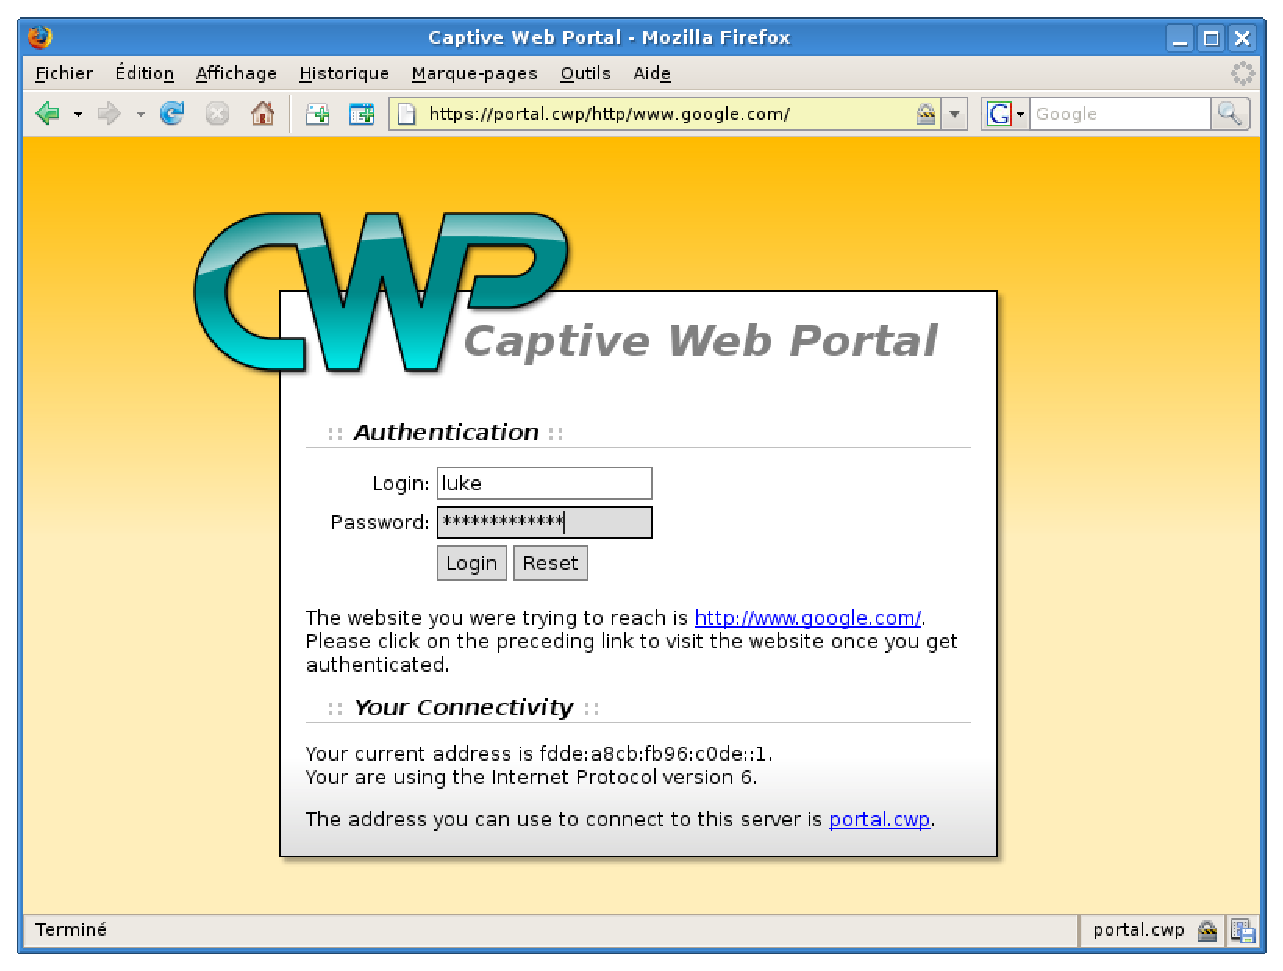
\includegraphics[keepaspectratio,width=0.67\textwidth]{images/screenshot}
\end{center}

\end{document}
